\section{Evaluation}

\begin{figure}[!ht]
    \centering
    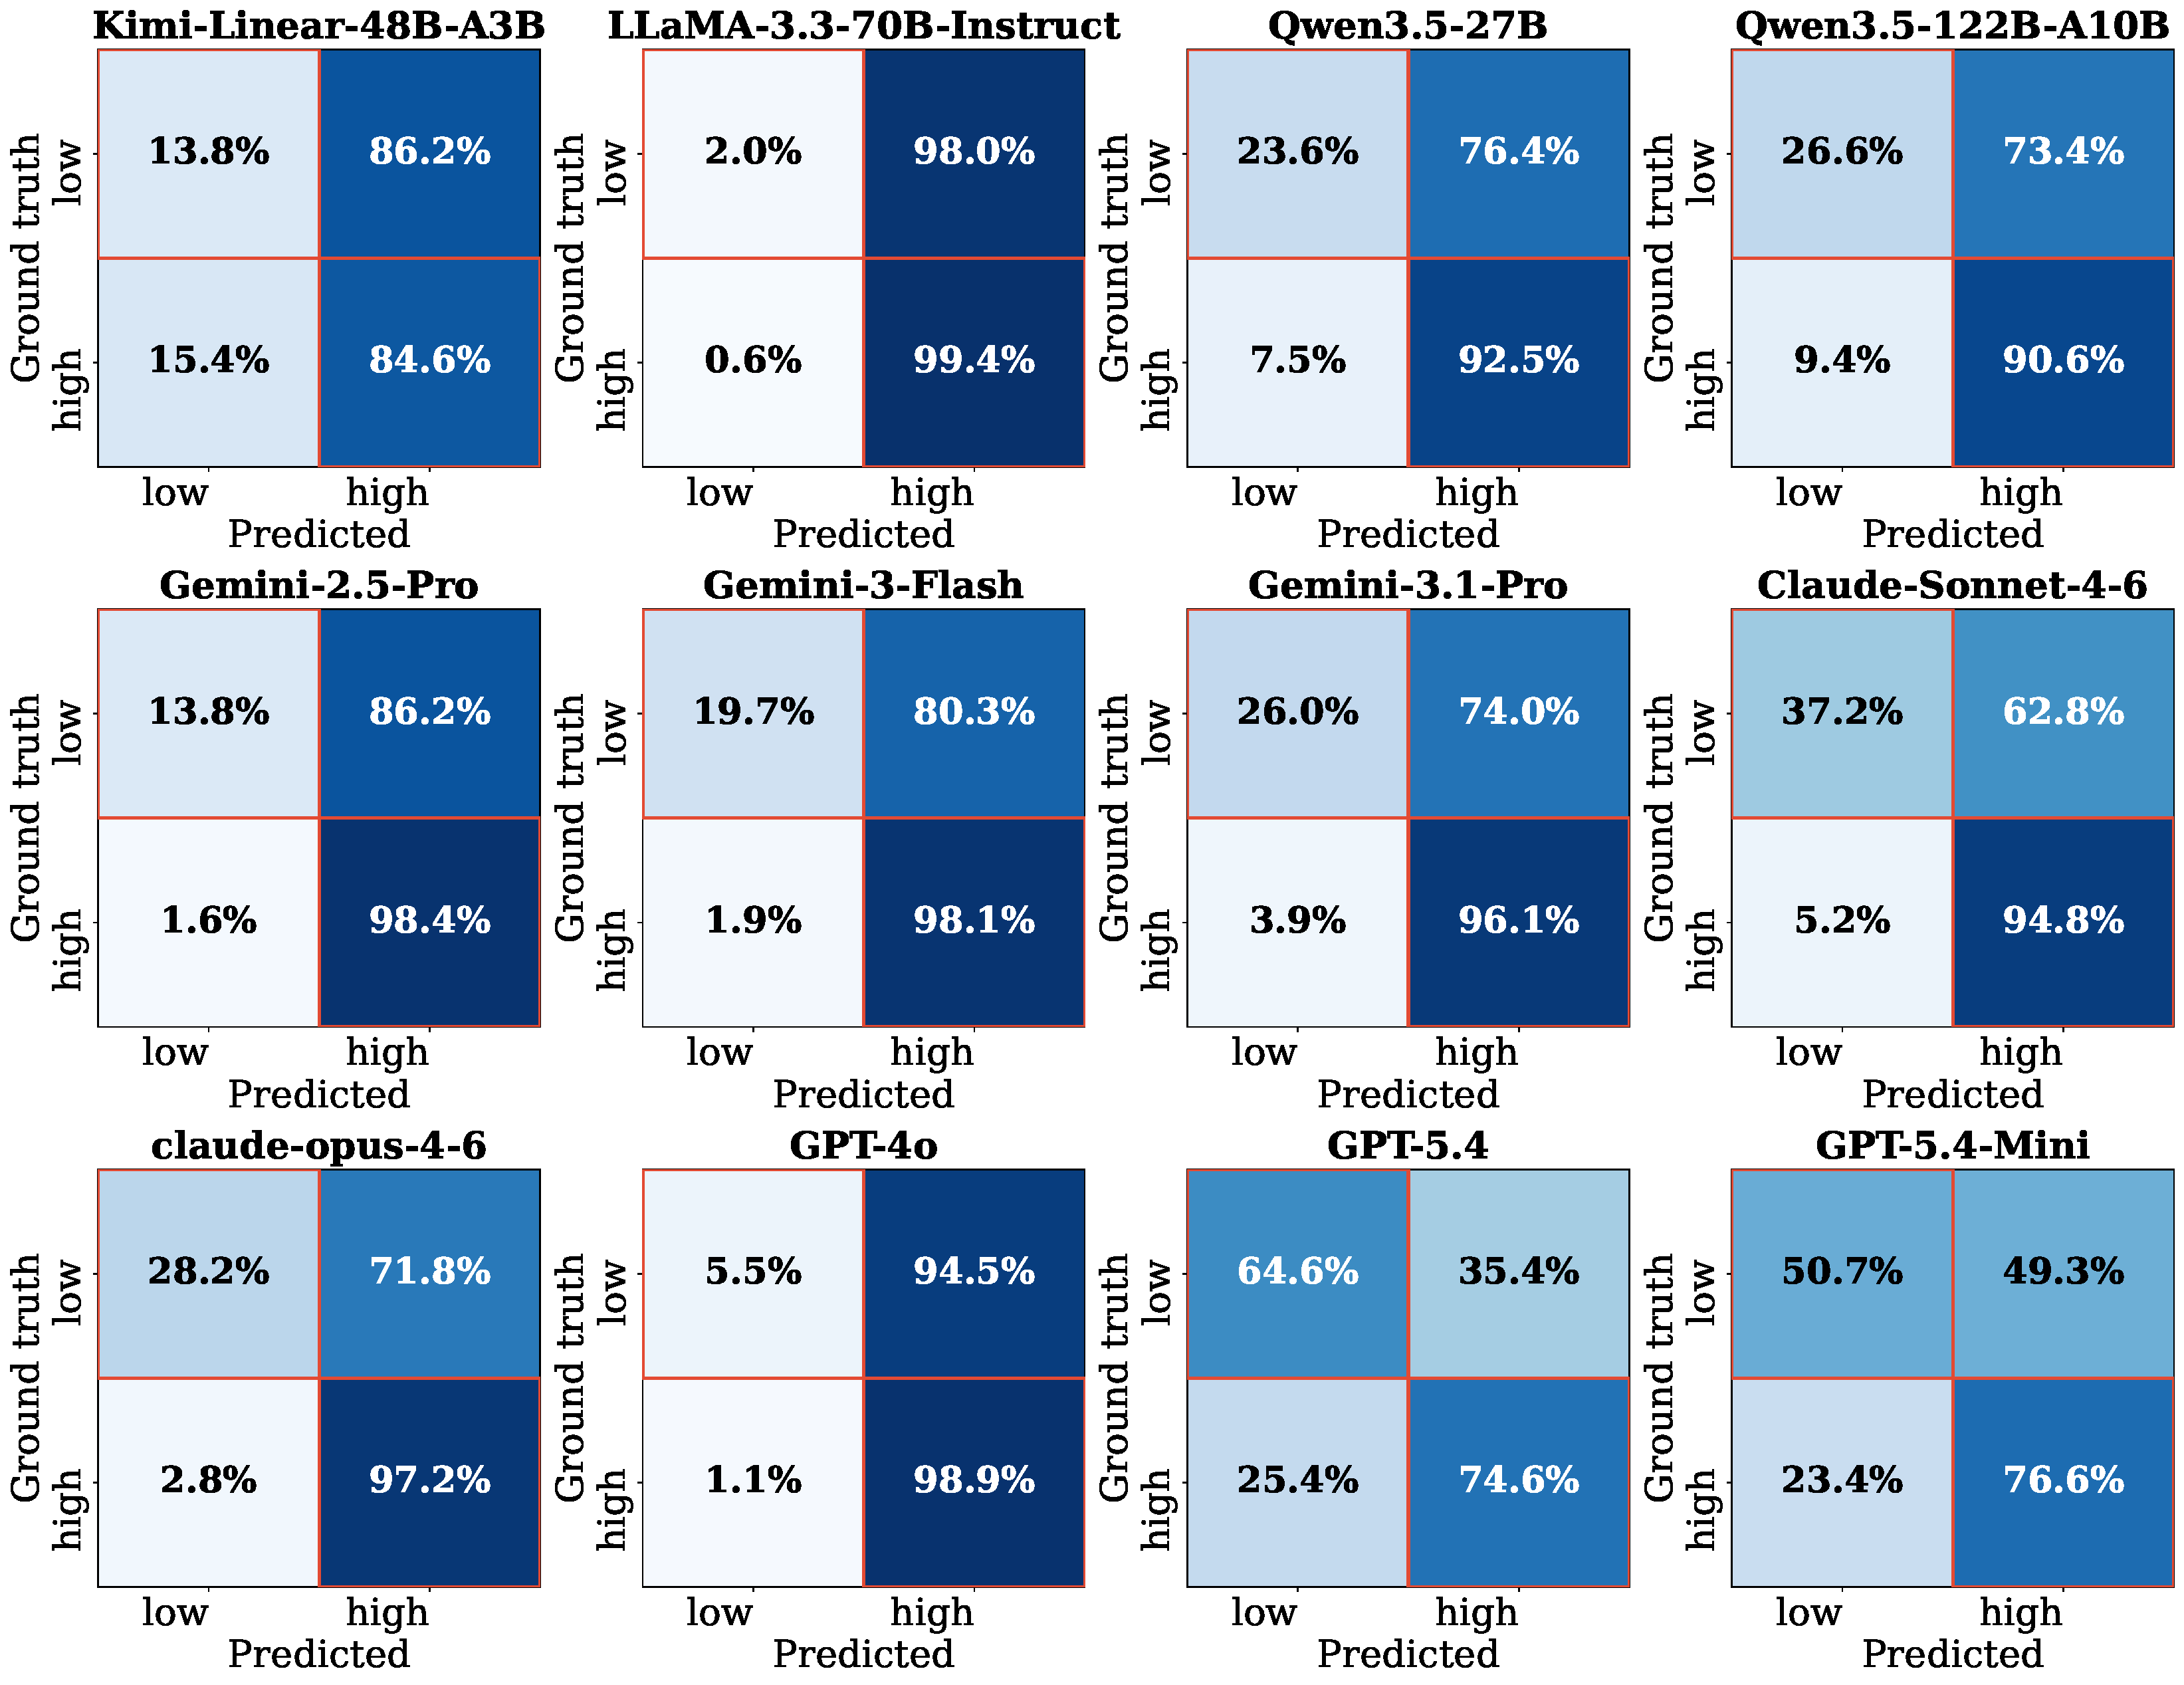
\includegraphics[width=0.95\linewidth,trim=0 0 0 0,clip]{figures/eval_confusion_all.pdf}
    \caption{Confusion matrices under the standard prompt across 12 evaluated models. Main message: many models are overoptimistic by default. The mean false-positive rate on low-soundness proposals is 74.0\% (9/12 models exceed 70\%). This pattern appears across model families in this evaluation setting.}
    \label{fig:eval-confusion-standard}
\end{figure}

% This section is organized as follows: we first describe the evaluation protocol, models, and metrics (Sec.~\ref{sec:eval:setup}); then present the main results under standard prompting (Sec.~\ref{sec:eval:main-results}); and finally analyze how aggressive prompting changes model behavior and calibration (Sec.~\ref{sec:eval:aggressive}).
This section is organized as follows: we first describe the evaluation protocol, models, and metrics (Sec.~\ref{sec:eval:setup}); then present the main results under standard prompting (Sec.~\ref{sec:eval:main-results}); summarize robustness controls for leakage, contamination, and shallow confounders (Sec.~\ref{sec:eval:controls}); and finally analyze how aggressive prompting changes model behavior and calibration (Sec.~\ref{sec:eval:aggressive}).

\subsection{Evaluation Setup}\label{sec:eval:setup}

We evaluate frontier large language models on SoundnessBench, which is built from real ML research submissions and targets recoverable proposal-stage methodological soundness rather than exact full-paper review prediction. In each test, we provide a results-masked research proposal to an LLM with a fixed evaluation prompt. The model is asked to classify the proposal as high or low soundness and provide a justification before the final label.

\textbf{Models.}
We evaluate a diverse set of \textbf{12 frontier models} spanning small and large scales, non-reasoning and reasoning, and both closed- and open-source models. The evaluated set includes GPT models (GPT-4o, GPT-5.4-Mini, GPT-5.4), Claude models (Claude-Opus-4.6, Claude-Sonnet-4.6), Gemini models (Gemini-2.5-Pro, Gemini-3-Flash, Gemini-3.1-Pro), Qwen models (Qwen-3.5-27B, Qwen-3.5-122B-A10B), a LLaMA model (LLaMA-3.3-70B), and a Kimi model (Kimi-Linear-48B-A3B).

\textbf{Inference Setup.}
For closed-source models, we run inference through the corresponding provider APIs. For open-source models, we deploy model servers with vLLM on 2$\times$NVIDIA H200 GPUs. Unless otherwise noted, we use a consistent decoding configuration across models with \texttt{max\_tokens=8192} and \texttt{temperature=0.2}; other generation parameters follow framework/provider defaults.



\textbf{Prompting Protocol.}
We evaluate each model under two prompting regimes:
\begin{itemize}[leftmargin=*,itemsep=0in, topsep=0in, parsep=0in]
    \item \textbf{Standard prompt.} This evaluation mode asks models to assess proposal soundness with a structured justification before the final classification, without imposing an explicit conservative prior.
    \item \textbf{Aggressive prompt.} Motivated by the optimism bias observed under the standard prompt, this stricter stress test instructs models to default to \textit{low soundness} unless the idea and experimental design are clearly strong and well-justified.
\end{itemize}

This setup lets us probe whether models possess a stable notion of proposal-stage methodological soundness, or whether their judgments are sensitive to prompt framing. We do not claim to exhaust the space of possible prompts; rather, the two prompts test whether a standard justification-first prompt and a deliberately stricter prompt can jointly preserve discrimination on both classes. Data-construction prompts are documented in Supplementary Sec.~\ref{sec:supp:data-construction}, and additional evaluation analyses are provided in Supplementary Sec.~\ref{sec:supp:evaluation}.



\textbf{Metrics.}
We report confusion matrices over the binary classification task, evaluating the ability to (i) reject low-soundness ideas and (ii) correctly identify high-soundness ones. An ideal model should concentrate on the diagonal entries (low$\rightarrow$low and high$\rightarrow$high), with both low false-positive rates on low-soundness proposals and low false-negative rates on high-soundness proposals. Off-diagonal errors indicate failure modes: optimism bias (low$\rightarrow$high) or over-conservatism (high$\rightarrow$low). We also report class-wise recall for both labels (Low R and High R) and Macro F1 (the unweighted average of per-class F1 scores).



\subsection{Main Results: A Broad Optimism Bias in Scientific Judgment}\label{sec:eval:main-results}\label{Sec: Main Results: Consistent Optimism Bias in Scientific Assessment}



\begin{table}[!htbp]
\centering
% \renewcommand{\arraystretch}{1.0}
\caption{Summary evaluation metrics across 12 models under standard and aggressive 
prompting. Low R and High R denote recall on low- and 
high-soundness proposals. Macro F1 is the unweighted average of 
per-class F1 scores. Best Macro F1 per condition is \textbf{bolded}. 
$\dagger$ denotes reasoning model.}
\label{tab:main_results}
\resizebox{0.9\textwidth}{!}{%
\begin{tabular}{lcccccc}
\toprule
& \multicolumn{3}{c}{\textbf{Standard Prompt}} 
& \multicolumn{3}{c}{\textbf{Aggressive Prompt}} \\
\cmidrule(lr){2-4} \cmidrule(lr){5-7}
\textbf{Model} 
& \textbf{Low R} $\uparrow$ & \textbf{High R} $\uparrow$ & \textbf{Macro F1} $\uparrow$
& \textbf{Low R} $\uparrow$ & \textbf{High R} $\uparrow$ & \textbf{Macro F1} $\uparrow$ \\
\midrule
\multicolumn{7}{l}{\textit{Open-source Models}} \\
LLaMA-3.3-70B          & 2.0  & 99.4 & 38.9 & 39.3 & 76.1 & 57.5 \\
Kimi-Linear-48B-A3B    & 13.8 & 84.6 & 44.6 & 50.2 & 45.8 & 47.5 \\
Qwen3.5-27B$^\dagger$  & 23.6 & 92.5 & 55.1 & 83.8 & 32.4 & 52.6 \\
Qwen3.5-122B-A10B$^\dagger$ & 26.6 & 90.6 & 56.3 & 95.6 & 16.8 & 44.7 \\
\midrule
\multicolumn{7}{l}{\textit{Closed-source Models}} \\
GPT-4o$^\dagger$       & 5.5  & 98.9 & 42.3 & 87.1 & 25.0 & 48.5 \\
GPT-5.4-mini           & 50.7 & 76.6 & 63.8 & 100.0 & 0.2 & 29.7 \\
GPT-5.4$^\dagger$      & 64.6 & 74.6 & \textbf{69.7} & 100.0 & 0.0 & 29.5 \\
Gemini-2.5-Pro$^\dagger$         & 13.8 & 98.4 & 49.8 & 73.4 & 55.1 & 62.7 \\
Gemini-3-Flash         & 19.7 & 98.1 & 54.5 & 76.4 & 60.4 & 67.1 \\
Gemini-3.1-Pro$^\dagger$         & 26.0 & 96.1 & 58.4 & 89.1 & 35.9 & 57.0 \\
Claude-Sonnet-4.6$^\dagger$      & 37.2 & 94.8 & 65.3 & 94.4 & 18.8 & 46.0 \\
Claude-Opus-4.6$^\dagger$        & 28.2 & 97.2 & 60.5 & 72.2 & 66.4 & \textbf{68.6} \\
\midrule
\textbf{Mean}          & 26.0 & 91.8 & 54.9 & 80.1 & 36.1 & 49.3 \\
\bottomrule
\end{tabular}%
}
\end{table}

\fh{\textit{Across LLM families, we observe a pervasive optimism bias: models frequently rate proposals with low reviewer-derived soundness labels as sound.}} As summarized in Tab.~\ref{tab:main_results} and visualized in Fig.~\ref{fig:eval-confusion-standard}, many proposals labeled as low soundness are predicted as high soundness. Specifically, under standard prompting, mean low-soundness recall is 26.0\% (equivalently, a 74.0\% false-positive rate), while mean high-soundness recall remains 91.8\%. At the model level, 9/12 models (including Gemini-3.1-Pro and Claude-Opus-4.6) label more than 70\% of low-soundness proposals as high soundness. The strongest optimism appears in LLaMA-3.3-70B and GPT-4o, which classify 98.0\% and 94.5\% of low-soundness proposals as high soundness. This pattern indicates that model judgments are often skewed toward approval even when proposal quality is limited. In practice, many default model configurations behave as permissive first-gate reviewers. Instead of consistently filtering weak proposals, they approve a broad set of candidates, which can lead to avoidable compute spend and weaker downstream experimentation. \tuyen{Representative false-positive and true-positive examples, together with concrete model responses, are provided in Supplementary Sec.~\ref{sec:supp:qualitative-fp-tp}.}

\textit{A few frontier LLMs reduce optimism bias, but at the cost of missing more high-soundness proposals.} For example, GPT-5.4 and GPT-5.4-mini are more conservative, but their high-soundness recall drops to 74.6\% and 76.6\%, respectively. \fh{This suggests a calibration trade-off in current frontier LLMs for proposal-stage soundness judgment: stricter filtering can suppress false approvals, but it also increases the risk of rejecting promising ideas.}

\begin{figure}[t]
    \centering
    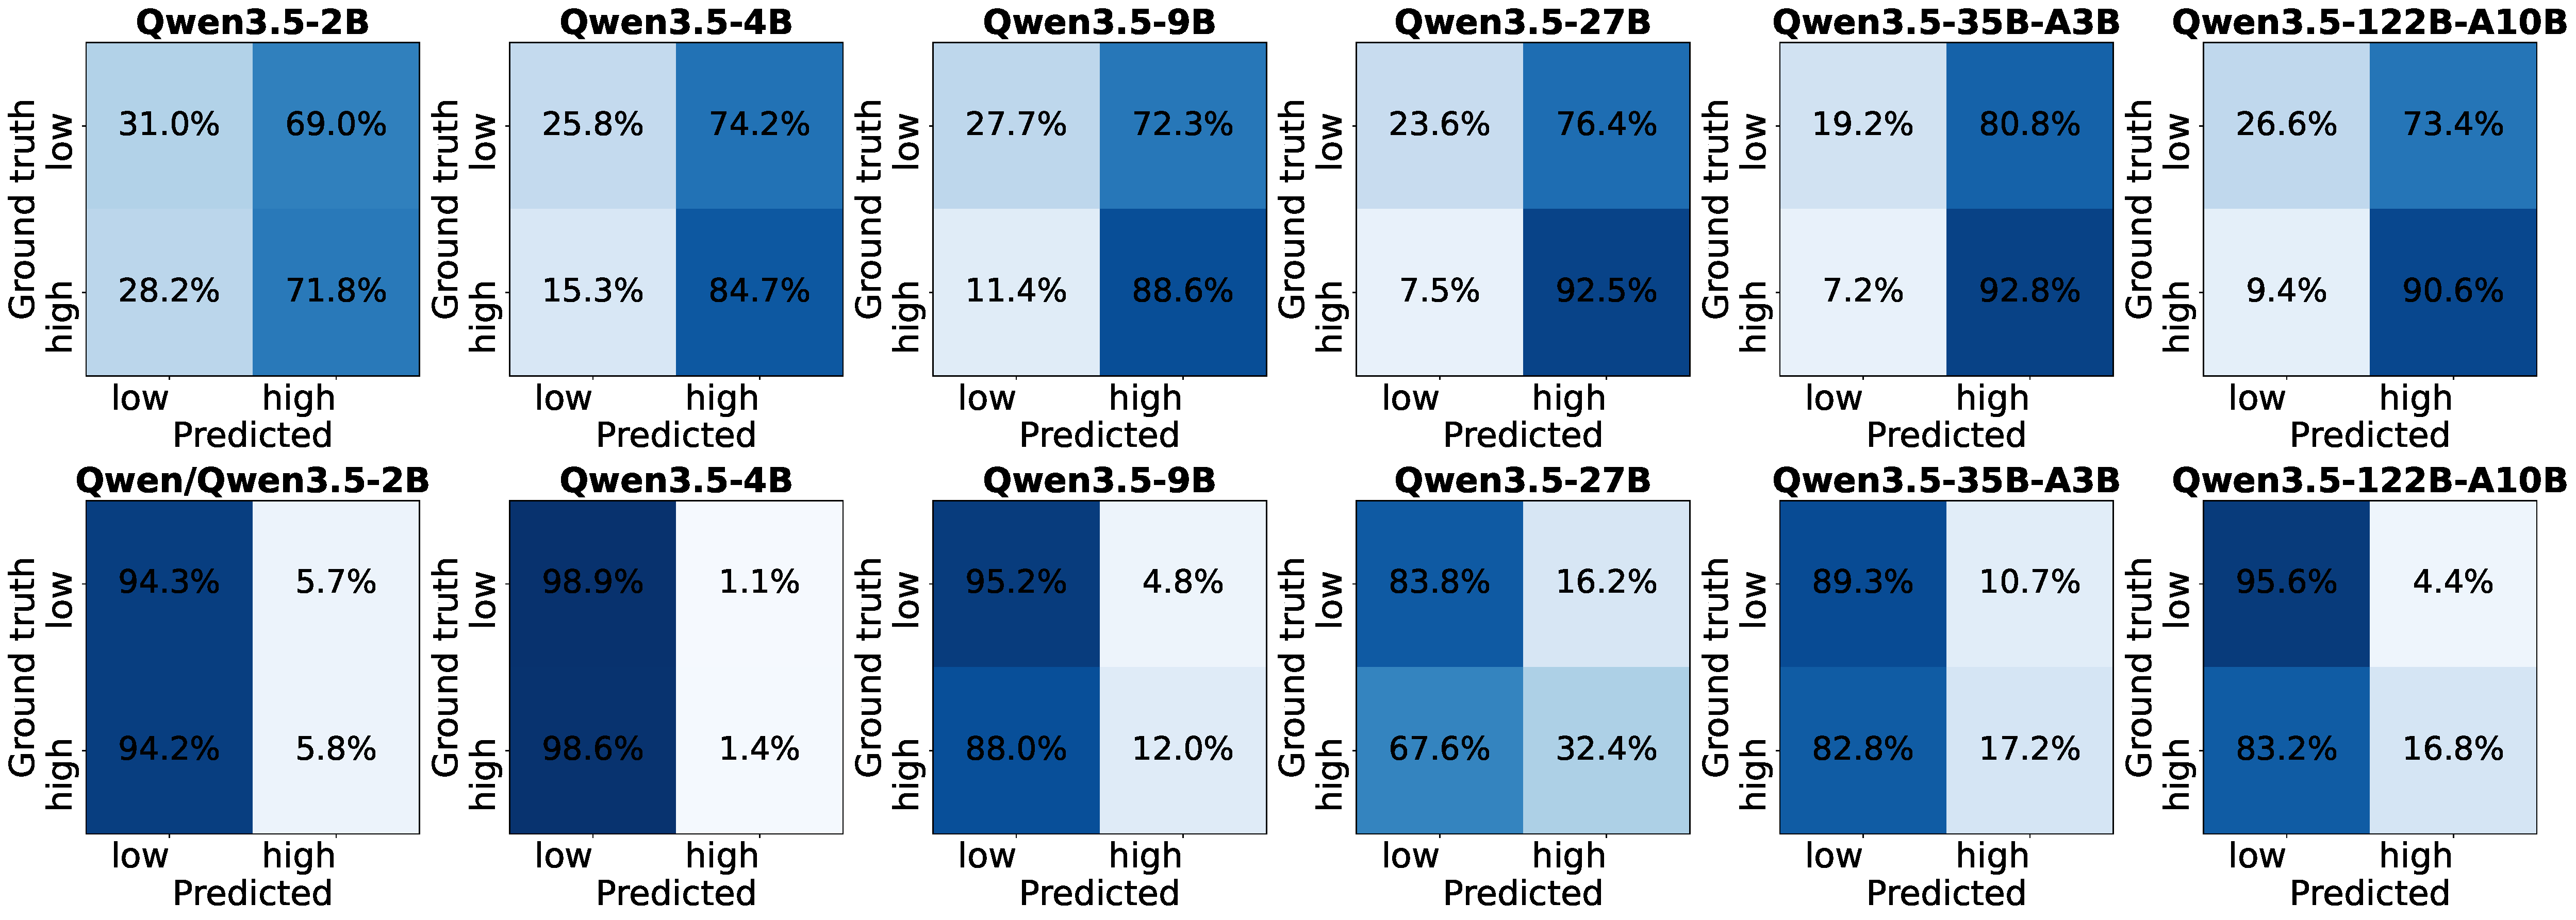
\includegraphics[width=\linewidth]{figures/scale_confusion_merged.pdf}
    \caption{Confusion matrices across six Qwen3.5 model sizes
    (2B--122B) under standard \textbf{(top)} and aggressive \textbf{(bottom)} prompting. Under standard prompting, high-soundness recall improves with scale but low-soundness recall degrades. Larger models become more optimistic. Under aggressive prompting, models shift toward over-conservatism with no consistent improvement from scale.}
    \label{fig:scale}
\end{figure}

\fh{\textit{The optimism bias is not simply a small-model artifact.} To isolate scale from model family and training recipe, we evaluate six models from the same Qwen3.5 family, ranging from 2B to 122B parameters, under both prompting conditions (Fig.~\ref{fig:scale}). Under standard prompting, high-soundness recall improves with scale (71.8\% at 2B to 92.8\% at 35B), but low-soundness recall simultaneously decreases (31.0\% at 2B to 19.2\% at 35B). In other words, larger models become \textit{more} permissive toward weak proposals, not less. Under aggressive prompting, scale also provides no consistent recovery: all six models trend toward over-conservatism, with high-soundness recall ranging from 1.4\% (4B) to 32.4\% (27B) and no monotonic improvement with size.}



\subsection{\fh{Robustness Controls and Alternative Explanations}}\label{sec:eval:controls}

\fh{Because SoundnessBench is reconstructed from public ICLR papers and uses reviewer-derived soundness labels, we explicitly test whether the main optimism-bias pattern could be explained by label noise, extraction leakage, public-corpus contamination, paper recognition, shallow textual structure, or slice-level concentration. These controls do not make the benchmark contamination-free or convert reviewer scores into perfect ground truth; instead, they narrow the most plausible alternative explanations for the observed behavior.}

\begin{table}[t]
\centering
\caption{\fh{Reduced-contamination-risk check using an ICLR 2026-only split. We evaluate the standard prompt on the subset of models with documented training cutoffs before the ICLR 2026 submission period, then compare their mean predictions on the full dataset and on the ICLR 2026-only split. The main observation is that the optimism bias remains stable under this reduced-contamination-risk setting: low-soundness proposals are still predicted as high soundness at a similar rate on the 2026-only split and the full dataset.}}
\label{tab:contamination_2026}
\resizebox{0.6\linewidth}{!}{%
\begin{tabular}{lcc}
\toprule
\fh{\textbf{Ground Truth / Split}} & \fh{\textbf{Predicted Low}} & \fh{\textbf{Predicted High}} \\
\midrule
\fh{Low (Full Dataset)} & \fh{26.12\%} & \fh{73.88\%} \\
\fh{Low (ICLR 2026 Only)} & \fh{22.53\%} & \fh{77.47\%} \\
\fh{High (Full Dataset)} & \fh{8.14\%} & \fh{91.86\%} \\
\fh{High (ICLR 2026 Only)} & \fh{7.77\%} & \fh{92.23\%} \\
\bottomrule
\end{tabular}%
}
\end{table}



\begin{itemize}[leftmargin=*,itemsep=0in, topsep=0in, parsep=0in]
    \item \fh{\textbf{Label and leakage audit.} A preliminary human verification audit checks whether extracted proposals leak results or outcome cues and whether reviewer-derived labels are defensible from the proposal and source document. In the completed audited subset, 92.3\% of leakage checks match the expected ``No'' answer and 84.6\% of label-validity checks match the expected ``Yes'' answer (Supplementary Sec.~\ref{sec:supp:human-audit}).}
    \item \fh{\textbf{Contamination and identifier controls.} As shown in Tab.~\ref{tab:contamination_2026}, on an ICLR 2026-only split evaluated with cutoff-restricted models, low-soundness proposals are still predicted as high soundness at a similar rate to the full dataset (77.47\% vs. 73.88\%). Removing paper-identifying phrases changes the aggregate confusion matrix by roughly one percentage point (Supplementary Sec.~\ref{sec:supp:contamination-control}, Sec.~\ref{sec:supp:identifier-removal}).}
    \item \fh{\textbf{Surface-feature and slice controls.} Simple no-training baselines based on proposal length, experiment count, and risk-factor count fail in the opposite direction from LLMs: they over-reject high-soundness proposals, whereas LLMs over-approve low-soundness proposals. The optimism bias also persists across years, subfields, and writing-quality bands (Supplementary Sec.~\ref{sec:supp:surface-baselines}, Sec.~\ref{sec:supp:slice-breakdowns}).}
    \item \fh{\textbf{Adversarial content control.} When severe hypothesis--experiment mismatches are injected into 100 high-soundness proposals, GPT-5.4's approval rate drops from 77.0\% to 1.0\%, suggesting that models do attend to salient methodological content but remain insufficiently critical of subtler naturally occurring flaws (Supplementary Sec.~\ref{sec:supp:adversarial-injection}).}
\end{itemize}

\fh{Overall, these analyses support a calibrated interpretation: SoundnessBench is an imperfect but audited proxy for recoverable proposal-stage soundness, and the observed optimism bias is unlikely to be explained solely by leakage, memorization, simple style features, or a narrow topic slice.}

\begin{figure}[t]
    \centering
    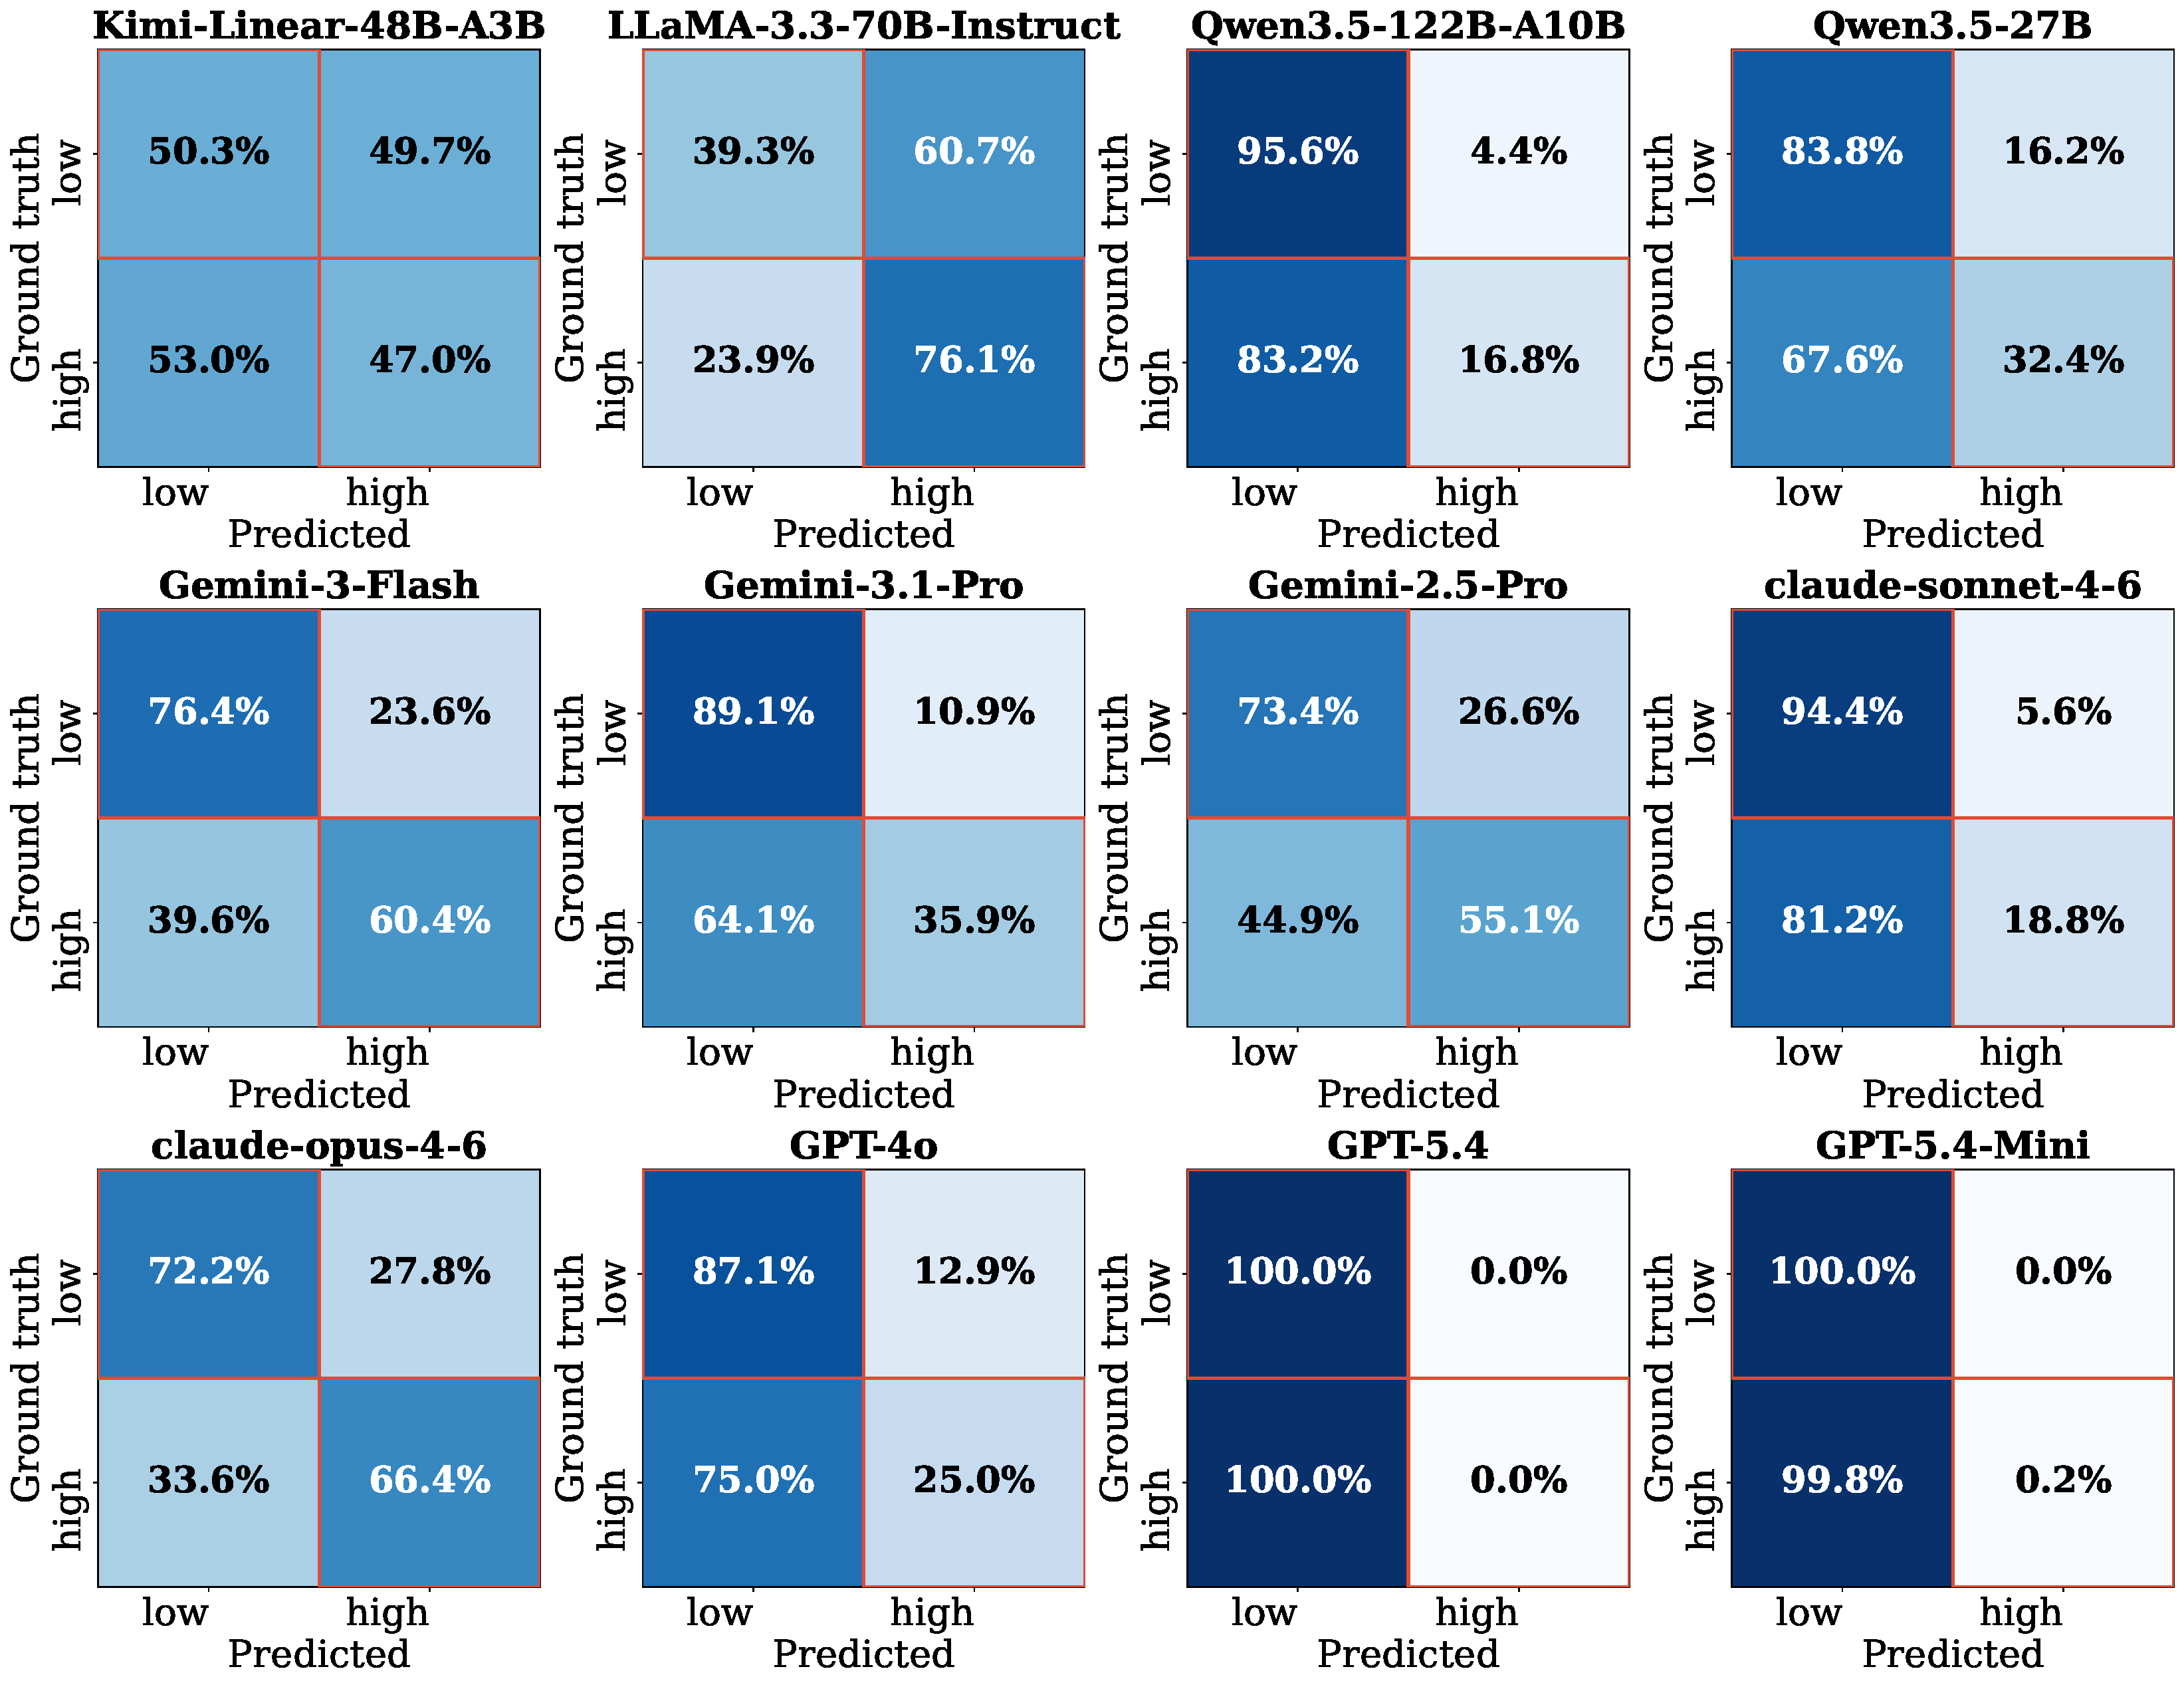
\includegraphics[width=0.95\linewidth,trim=0 12 0 0,clip]{figures/eval_confusion_aggressive_all.pdf}
    \caption{Confusion matrices under the aggressive prompt across 12 evaluated models. Main message: optimism bias often shifts toward over-conservatism. The mean false-positive rate on low-soundness proposals drops to 19.9\% (10/12 models are below 30\%), but recall on high-soundness proposals also drops to 36.1\% (7/12 models are below 40\%). This illustrates strong prompt sensitivity in proposal-stage soundness judgment for the evaluated models.}
    \label{fig:eval-confusion-aggressive}
\end{figure}



\subsection{Under Aggressive Prompting: Bias Shifts Toward Over-Conservatism}\label{sec:eval:aggressive}\label{Sec: Under Aggressive Prompting: Optimism Bias Is Not Fixed, It Is Inverted}

\fh{\textit{The tested stricter prompt does not jointly improve both classes; it mainly shifts errors from false positives to false negatives.}} We observe widespread optimism bias in Sec.~\ref{sec:eval:main-results}. Motivated by this, we test how judgments change when the decision threshold is made deliberately stricter while keeping the same models and task: default to \textit{low soundness} unless the idea and experimental design are clearly strong and well-justified. Additional analyses for this setting are presented in Supplementary Sec.~\ref{sec:supp:scale-bias} and Sec.~\ref{sec:supp:instruction-tuning-bias}. As shown in Tab.~\ref{tab:main_results} and Fig.~\ref{fig:eval-confusion-aggressive}, models generally become more conservative: low-soundness rejection improves, but high-soundness identification drops. The trade-off is quantitatively large. Mean low-soundness false positives drop from 74.0\% (standard prompt) to 19.9\% (aggressive prompt), and 10/12 models are below 30\%; meanwhile, mean high-soundness recall drops from 91.8\% to 36.1\%, with 7/12 models below 40\%. At the extreme, GPT-5.4 and GPT-5.4-Mini move to near-always-low behavior under aggressive prompting: low-soundness false positives are 0\% for both, while high-soundness recall falls to 0.0\% and 0.2\%, respectively. Other models show the same pattern in milder form; for example, Qwen3.5-122B-A10B and Claude-Sonnet-4.6 strongly reject low-soundness ideas (95.6\% and 94.4\% rejection), but correctly identify only 16.8\% and 18.8\% of high-soundness proposals. Consistent with this, mean Macro F1 decreases from 54.9 to 49.3.

\fh{\textit{Taken together, these results point to a prompt-sensitive capability limitation in proposal-stage judgment.}} Prompt sensitivity varies substantially across models. Remarkably, GPT-5.4 has the best Macro F1 under standard prompting (69.7\%) but drops sharply under aggressive prompting (29.5\%), whereas Claude-Opus-4.6 changes much less (60.5\% vs.\ 68.6\%). This cross-model variation, together with the robustness analyses (Sec.~\ref{sec:eval:controls}; Supplementary Sec.~\ref{sec:supp:instruction-tuning-bias} and Sec.~\ref{sec:supp:scale-bias}), suggests that the optimism bias is prompt-sensitive, persists across tested model scales, and is not removed by instruction tuning within the examined family.



\begin{tcolorbox}[colback=green!5,colframe=teal!60!black,boxrule=0.8pt]
\fh{\textit{\textbf{Key Takeaway 1.}} Frontier LLMs show a broad optimism bias: models frequently rate low-soundness proposals as sound under standard prompting.} 

\medskip
\fh{\textit{\textbf{Key Takeaway 2.}} The tested stricter prompt does not jointly improve discrimination on both classes; it mainly shifts errors from false positives to false negatives.}

\medskip
\fh{\textit{\textbf{Key Takeaway 3.}} Taken together, results point to a prompt-sensitive capability limitation in proposal-stage soundness judgment: current LLMs are not yet reliable as standalone gatekeepers for scientific rigor.}
\end{tcolorbox}